\section{The CLI JIT backend}
\label{sec:clibackend}

\subsection{JIT layering}

From the implementation point of view, the JIT generator is divided into a
frontend and several backends.  The goal of the frontend is to generate a JIT
compiler which works as described in the previous sections.  Internally, the
JIT represents the compiled code as \emph{flow graphs}, and the role of
the backends is to translate flowgraphs into machine code.

At the moment of writing, three backends have been implemented: one for Intel
\emph{x86} processors, one for \emph{PowerPC} processors, and one for the
\emph{CLI Virtual Machine}.  The latter is special because instead of emitting
code for a real CPU it emits code for a virtual machine\footnote{By using the 
\lstinline{Reflection.Emit} namespace and creating \lstinline{DynamicMethod}s.}: 
before being executed, the generated code will be compiled again by the .NET JIT
compiler.

Thus, when using the CLI backend, we actually have two JIT compilers at two different
layers, each one specialized in different kinds of optimization.
By operating at a higher level, our JIT can potentially do a better job 
in some contexts, as our benchmarks demonstrate (see
Section~\ref{sec:benchmarks}).  On the other hand, the lower-level .NET JIT is
very good at producing machine code, much more than PyPy's own \emph{x86}
backend, for example.  By combining the strengths of both we can get highly
efficient machine code.

As usual, the drawback is that programs that runs for a very short period of
time could run slower with JIT than without, due to the time spent doing the
initial (double) compilation.  
Finally, it is important to underline that while we have directed our efforts 
to generate a JIT compiler able to emit very efficient code,
the performance of the compiler itself has been neglected so far, but  
it is certainly an issue which will have to be considered in our future research.

\subsection{Flexswitches}

For a large part, implementing the CLI backend is easy and straightforward, as
there is a close correspondence between most of the operations used by
frontend's flowgraphs and the CLI instructions.  Thus, we will not go into
details for this part.

However the concept of \emph{flexswitch}, as described in
Section~\ref{sec:jitgen}, does not have any direct equivalent
in the CLI model, and it is hard to implement efficiently.

A flexswitch is a special kind of switch which can be dynamically
extended with new cases.  Intuitively, its behavior can be described
well in terms of flow graphs: a flexswitch can be considered 
as a special flow graph block where links to newly created blocks are
dynamically added whenever new cases are needed. 

\begin{figure}[h]
\begin{center}
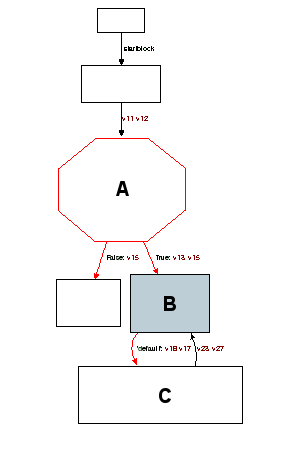
\includegraphics[height=5cm]{flexswitch1}
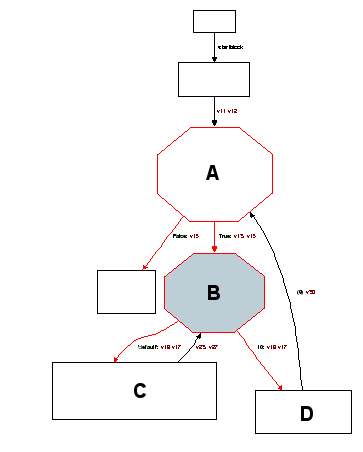
\includegraphics[height=5cm]{flexswitch2}
\caption{An example of a flexswitch evolution: in the picture on the
  right block D has been dynamically added.}\label{flexswitch-fig}
\end{center}
\end{figure}

In the pictures of Figure~\ref{flexswitch-fig}, block B (highlighted in grey)
corresponds to a flexswitch; initially (picture on the left) 
only block C, containing the code to restart the JIT compilation,
is connected to the flexswitch; the picture on the right
shows the graph after the first case has been dynamically added to the flexswitch,
by linking block B with the freshly created block D.


\subsection{Implementing flexswitches in CLI}
\label{sec:flexswitches-cli}

Implementing flexswitches for backends generating machine code is
not too complex: basically, a new jump has to be inserted in the
existing code to point to the newly generated code fragment.

Unfortunately, CLI does not allow modification of code which
has been already loaded and linked, therefore the simplest approach
taken for low level architectures does not work.

Since in .NET methods are the basic units of compilation, a possible
solution consists in creating a new method 
any time a new case has to be added to a flexswitch.

It is important to underline the difference between flow graphs and methods:
the first are the logical unit of code as seen by the JIT compiler, each of
them being concretely implemented by \emph{one or more} methods.

In this way, whereas flow graphs without flexswitches are translated to a
single method, the translation of \emph{growable} flow graphs will be
scattered over several methods.  Summarizing, the backend behaves in the
following way:
\begin{itemize}
\item Each flow graph is translated in a collection of methods which
  can grow dynamically. Each collection contains at least one
  method, called \emph{primary}, which is the first to be created.
  All other methods, called \emph{secondary}, are added dynamically 
  whenever a new case is added to a flexswitch.

\item Each either primary or secondary method implements a certain
  number of blocks, all belonging to the same flow graph.
\end{itemize} 

When a new case is added to a flexswitch, the backend generates the new blocks
into a new single method.  The newly created method is pointed to by a
delegate\footnote{\emph{Delegates} are the .NET equivalent of function
  pointers.} stored in the flexswitch, so that it can be invoked later when
needed.

\subsubsection{Internal and external links}

A link is called \emph{internal} if it connects two blocks implemented
by the same method,
\emph{external} otherwise.

Following an internal link is easy in IL bytecode: a jump to
the corresponding code fragment in the same method can be emitted 
to execute the new block, whereas the appropriate local variables can be
used for passing arguments. 

Following an external link whose target is an initial block could also
be easily implemented, by just invoking the corresponding method.
What cannot be easily implemented in CLI is following an external link
whose target is not an initial block; consider, for instance, the
outgoing link from block D to block A in Figure~\ref{flexswitch-fig}. How is it possible to jump into
the middle of a method?

To solve this problem every method contains a special code, called
\emph{dispatcher}: whenever a method is invoked, its dispatcher is
executed first\footnote{The dispatcher should not be
confused with the initial block of a method.} to
determine which block has to be executed.
This is done by passing to the method a 32 bits number, called 
\emph{block id}, which uniquely identifies the next block of the graph to be executed.
The high 2 bytes of a block id constitute the \emph{method id}, which 
univocally identifies a method in a graph, whereas the low 2 bytes constitute
a progressive number univocally identifying a block inside each method.

The picture in Figure~\ref{block-id-fig} shows a graph composed of three methods (for
simplicity, dispatchers are not shown); method ids are in bold, whereas
block numbers are in black. 
The graph contains three external links; in particular, note the link
between blocks \texttt{0x00020001} and \texttt{0x00010001} which
connects two blocks implemented by different methods.
\begin{figure}[h]
\begin{center}
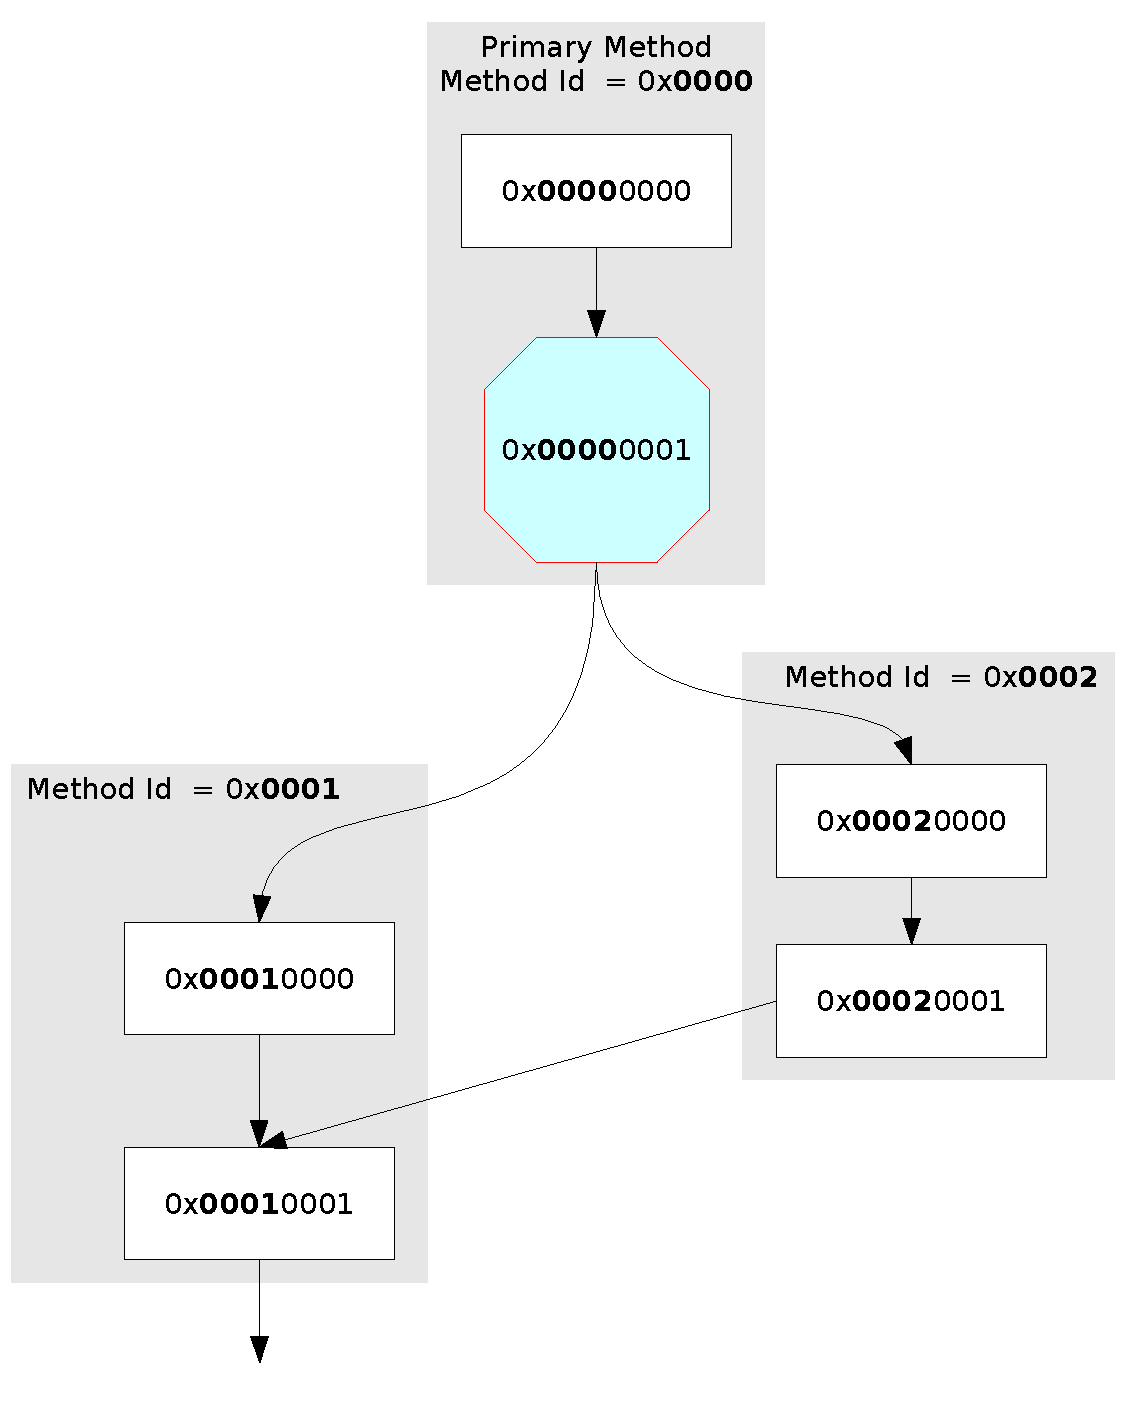
\includegraphics[height=6cm]{blockid}
\caption{Method and block ids.}\label{block-id-fig}
\end{center}
\end{figure}

The code\footnote{For simplicity we write C\# code instead of
the actual IL bytecode.} generated for the dispatcher of methods
is similar to the following fragment: 
\begin{lstlisting}[language={[Sharp]C}]
// dispatch block
int methodid = (blockid && 0xFFFF0000) >> 16; 
int blocknum = blockid && 0x0000FFFF;         
if (methodid != MY_METHOD_ID) {
  // jump_to_ext 
  ...
}
switch(blocknum) {
  case 0: goto block0;
  case 1: goto block1;
  default: throw new Exception("Invalid block id");
}
\end{lstlisting}
If the next block to be executed is implemented in the same method
(\lstinline{methodid == MY_METHOD_ID}), then the appropriate
jump to the corresponding code is executed.
Otherwise, the \lstinline{jump_to_ext}
part of the dispatcher has to be executed, which is implemented differently 
by primary and secondary methods.

The primary method is responsible for the bookkeeping of the secondary
methods which are added to the same graph dynamically. This can be 
simply implemented with an array mapping method id of secondary methods
to the corresponding delegate. Therefore, the primary methods contain
the following \lstinline{jump_to_ext} code (where
\lstinline{FlexSwitchCase} is the type of delegates for secondary methods):
\begin{lstlisting}[language={[Sharp]C}] 
// jump_to_ext
FlexSwitchCase meth = method_map[methodid];
blockid = meth(blockid, ...); // execute the method
goto dispatch_block;
\end{lstlisting}
Each secondary method returns the block id of the next block to be
executed; therefore, after the secondary method has returned, the
dispatcher of the primary method will be executed again to jump
to the correct next block. 

To avoid mutual recursion and an undesired growth of the stack,
the \lstinline{jump_to_ext} code in dispatchers of secondary methods
just returns the block id of the next block; since the primary method
is always the first method of the graph which is called, the correct
jump will be eventually executed by the dispatcher of the primary method.

Clearly this complex translation is performed only for flow graphs
having at least one flexswitch; flow graphs without flexswitches
are implemented in a more efficient and direct way by a unique method
with no dispatcher.

\subsubsection{Passing arguments to external links}

The main drawback of our solution is that passing arguments across
external links cannot be done efficiently by using the parameters of
methods for the following reasons:
\begin{itemize}
\item In general, the number and type of arguments is different for every block in a graph;

\item The number of blocks of a graph can grow dynamically, therefore
  it is not possible to compute in advance the union of the arguments
  of all blocks in a graph; 

\item Since external jumps are implemented with a delegate, all the
  secondary methods of a graph must have the same signature.
\end{itemize}

Therefore, the solution we came up with is defining a class
\lstinline{InputArgs} for passing sequences of arguments whose length
and type is variable.
\begin{lstlisting}[language={[Sharp]C}] 
public class InputArgs {
  public int[] ints;
  public float[] floats;
  public object[] objs;
  ...
}
\end{lstlisting}
Unfortunately, with this solution passing arguments to external links
becomes quite slow:
\begin{itemize}
\item When writing arguments, array re-allocation may be needed in
  case the number of arguments exceeds the dimension of the
  array. Furthermore the VM will always perform bound-checks, even
  when the size is explicitly checked in advance;

\item When reading arguments, a bound-check is performed by the VM for
  accessing each argument; furthermore, an appropriate downcast must be
  inserted anytime an argument of type object is read.
\end{itemize}
Of course, we do not need to create a new object of class
\lstinline{InputArgs} any time we need to perform an external jump;
instead, a unique object is created at the beginning of the execution
of the primary method. 

\subsubsection{Implementation of flexswitches}

To implement each flexswitch, the CLI backend creates an instance of a subclass
of \lstinline{BaseLowLevelFlexSwitch}: such an instance stores the mapping
between each value and the corresponding method we want to invoke.  Then, the
generated code contains a call to the method \lstinline{execute}, which
selects and invoke the right method depending on the actual value we are
switching on.

The following snippet shows the special case of integer flexswitches:
\begin{lstlisting}[language={[Sharp]C}] 
public class IntLowLevelFlexSwitch: 
                        BaseLowLevelFlexSwitch {
  public uint default_blockid = 0xFFFFFFFF;
  public int numcases = 0;
  public int[] values = new int[4];
  public FlexSwitchCase[] cases = 
                          new FlexSwitchCase[4];

  public void add_case(int value, FlexSwitchCase c) {
    ...
  }

  public uint execute(int value, InputArgs args) {
    for(int i=0; i<numcases; i++)
      if (values[i] == value)
        return cases[i](0, args);
    return default_blockid;
  }
}
\end{lstlisting}

The mapping from integers values to delegates (pointing to secondary
methods) is just implemented by the two arrays \lstinline{values} and
\lstinline{cases}. Method \lstinline{add_case} extends the mapping
whenever a new case is added to the flexswitch.
  
The most interesting part is the body of method \lstinline{execute},
which takes a value and a set of input arguments to be passed across
the link and jumps to the right block by performing a linear search in
array \lstinline{values}\footnote{Our microbenchmarks indicate that a linear
search is the fastest way to find the right method to call, since typically
each flexswitch contains only a very small number of cases.}.

Recall that the first argument of delegate \lstinline{FlexSwitchCase} is the
block id to jump to. By construction, the target block of a flexswitch is
always the first in a secondary method, and we use the special value
\lstinline{0} to signal this.

The value returned by method \lstinline{execute} is the next block id
to be executed; 
in case no association is found for \lstinline{value},
\lstinline{default_blockid} is returned. The value of
\lstinline{default_blockid} is initially set by the JIT compiler and
usually corresponds to a block containing code to restart the JIT
compiler for creating a new secondary method with the new code for the
missing case, and updating the flexswitch by calling method
\lstinline{add_case}.

% LocalWords:  flexswitches backend flexswitch methodid blockid xFFFF blocknum
% LocalWords:  FFFF goto FlexSwitchCase meth InputArgs ints objs VM uint args
% LocalWords:  IntLowLevelFlexSwitch BaseLowLevelFlexSwitch xFFFFFFFF numcases
% LocalWords:  JIT
